% This file was created with tikzplotlib v0.10.1.
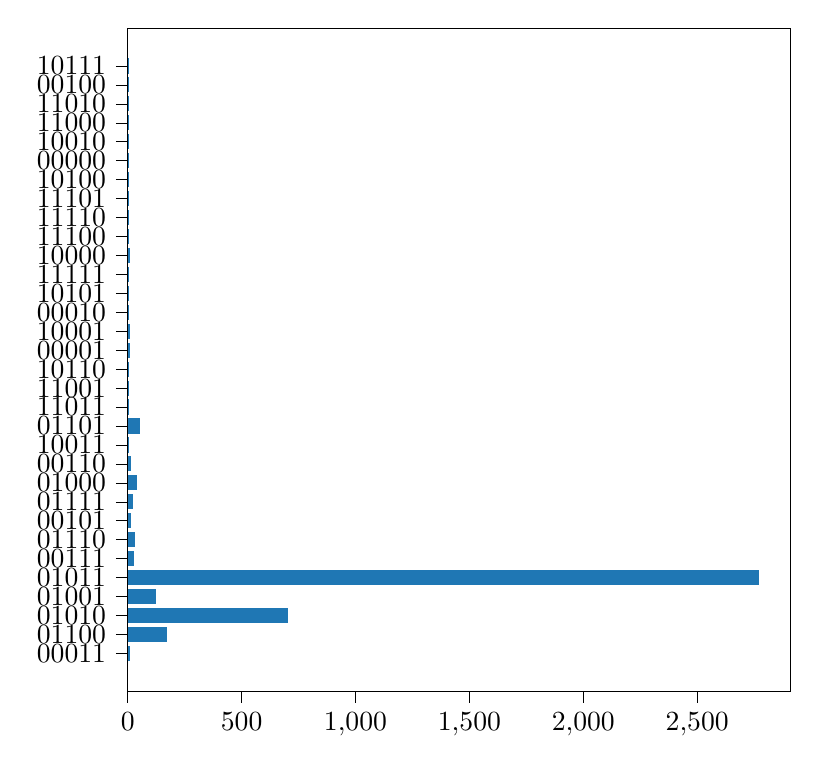
\begin{tikzpicture}

\definecolor{darkgray176}{RGB}{176,176,176}
\definecolor{steelblue31119180}{RGB}{31,119,180}

\begin{axis}[
height=10cm,
tick align=outside,
tick pos=left,
width=10cm,
x grid style={darkgray176},
xmin=0, xmax=2909.55,
xtick style={color=black},
y grid style={darkgray176},
ymin=-1.99, ymax=32.99,
ytick style={color=black},
ytick={0,1,2,3,4,5,6,7,8,9,10,11,12,13,14,15,16,17,18,19,20,21,22,23,24,25,26,27,28,29,30,31},
yticklabels={
  00011,
  01100,
  01010,
  01001,
  01011,
  00111,
  01110,
  00101,
  01111,
  01000,
  00110,
  10011,
  01101,
  11011,
  11001,
  10110,
  00001,
  10001,
  00010,
  10101,
  11111,
  10000,
  11100,
  11110,
  11101,
  10100,
  00000,
  10010,
  11000,
  11010,
  00100,
  10111
}
]
\draw[draw=none,fill=steelblue31119180] (axis cs:0,-0.4) rectangle (axis cs:10,0.4);
\draw[draw=none,fill=steelblue31119180] (axis cs:0,0.6) rectangle (axis cs:173,1.4);
\draw[draw=none,fill=steelblue31119180] (axis cs:0,1.6) rectangle (axis cs:704,2.4);
\draw[draw=none,fill=steelblue31119180] (axis cs:0,2.6) rectangle (axis cs:126,3.4);
\draw[draw=none,fill=steelblue31119180] (axis cs:0,3.6) rectangle (axis cs:2771,4.4);
\draw[draw=none,fill=steelblue31119180] (axis cs:0,4.6) rectangle (axis cs:28,5.4);
\draw[draw=none,fill=steelblue31119180] (axis cs:0,5.6) rectangle (axis cs:34,6.4);
\draw[draw=none,fill=steelblue31119180] (axis cs:0,6.6) rectangle (axis cs:15,7.4);
\draw[draw=none,fill=steelblue31119180] (axis cs:0,7.6) rectangle (axis cs:25,8.4);
\draw[draw=none,fill=steelblue31119180] (axis cs:0,8.6) rectangle (axis cs:42,9.4);
\draw[draw=none,fill=steelblue31119180] (axis cs:0,9.6) rectangle (axis cs:15,10.4);
\draw[draw=none,fill=steelblue31119180] (axis cs:0,10.6) rectangle (axis cs:8,11.4);
\draw[draw=none,fill=steelblue31119180] (axis cs:0,11.6) rectangle (axis cs:53,12.4);
\draw[draw=none,fill=steelblue31119180] (axis cs:0,12.6) rectangle (axis cs:2,13.4);
\draw[draw=none,fill=steelblue31119180] (axis cs:0,13.6) rectangle (axis cs:5,14.4);
\draw[draw=none,fill=steelblue31119180] (axis cs:0,14.6) rectangle (axis cs:4,15.4);
\draw[draw=none,fill=steelblue31119180] (axis cs:0,15.6) rectangle (axis cs:10,16.4);
\draw[draw=none,fill=steelblue31119180] (axis cs:0,16.6) rectangle (axis cs:11,17.4);
\draw[draw=none,fill=steelblue31119180] (axis cs:0,17.6) rectangle (axis cs:4,18.4);
\draw[draw=none,fill=steelblue31119180] (axis cs:0,18.6) rectangle (axis cs:4,19.4);
\draw[draw=none,fill=steelblue31119180] (axis cs:0,19.6) rectangle (axis cs:7,20.4);
\draw[draw=none,fill=steelblue31119180] (axis cs:0,20.6) rectangle (axis cs:11,21.4);
\draw[draw=none,fill=steelblue31119180] (axis cs:0,21.6) rectangle (axis cs:2,22.4);
\draw[draw=none,fill=steelblue31119180] (axis cs:0,22.6) rectangle (axis cs:4,23.4);
\draw[draw=none,fill=steelblue31119180] (axis cs:0,23.6) rectangle (axis cs:4,24.4);
\draw[draw=none,fill=steelblue31119180] (axis cs:0,24.6) rectangle (axis cs:5,25.4);
\draw[draw=none,fill=steelblue31119180] (axis cs:0,25.6) rectangle (axis cs:5,26.4);
\draw[draw=none,fill=steelblue31119180] (axis cs:0,26.6) rectangle (axis cs:5,27.4);
\draw[draw=none,fill=steelblue31119180] (axis cs:0,27.6) rectangle (axis cs:4,28.4);
\draw[draw=none,fill=steelblue31119180] (axis cs:0,28.6) rectangle (axis cs:1,29.4);
\draw[draw=none,fill=steelblue31119180] (axis cs:0,29.6) rectangle (axis cs:2,30.4);
\draw[draw=none,fill=steelblue31119180] (axis cs:0,30.6) rectangle (axis cs:2,31.4);
\end{axis}

\end{tikzpicture}
